\documentclass[10pt]{article}

\usepackage[margin = 1.5 cm]{geometry}
\usepackage{amsmath}
\usepackage{graphicx}
\usepackage{adjustbox}

\begin{document}
\section*{SWEN30006 - Project 3B Reflection}

\textbf{GROUP 19}

\subsection*{Design Changes \& Implementation}

\noindent Our initial application design would pre-calculate predictions up until the desired maximum time horizon every time a scraping operation had been completed. These predictions would then be stored in the database such that user forecast calls would simply be a look-up operation (plus some interpolation if the the call is made on a new location not already seeded into the database) rather than the slower process of having to compute a regression against existing data and fitting new points on call. \\\\
The main difficulty is anticipating user calls at times that don't coincide exactly with the times that the pre-generated predictions produce. To achieve this to within minute accuracy of the user call, minutely readings need to be predicted. For a maximum horizon of 180 minutes and approximately 75 seeded stations, predictions write time to the database becomes a bottleneck. Testing showed that computing predictions on call was sufficiently fast that it became a more attractive option given its ease of implementation and it does not necessitate a Prediction model, simplifying the overall application architecture. \\\\ 
To assist with returning Location attributes, Postcodes was changed from a Locations field to a separate model with Location associations i.e. Postcode has-many Locations and Location belongs-to Postcode. This would negate the need to  filter out locations by postcodes as they are now directly indexed. This would also reduce the number of calls made using the Google GeoCode API. \\\\
The changes to how postcodes are handled mean that postcode API calls no longer need to go through the Geocode API via the interpolator component and can now directly pull from the Postcode model. In the component diagram, this simply means that the interfaces need to change such that there are added associations between the Rails controller and Postcode tables in the SQLite Database. \\\\

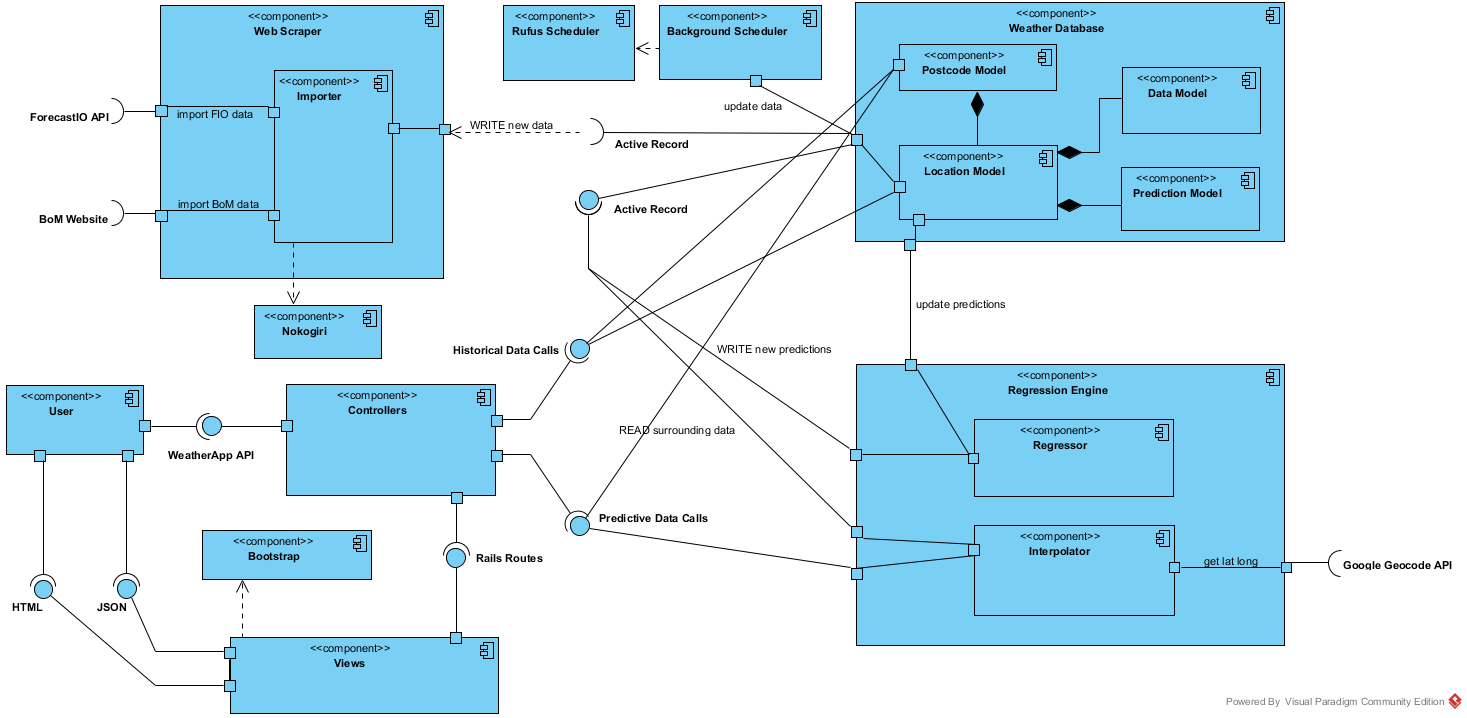
\includegraphics[scale=0.45]{P3_component_modified.png}

\newpage

\subsection*{Challenges}

\noindent One of the main challenges was working with the poor quality of data scraped from BoM (e.g. accumulated rainfall, overly discretised bearings, large gaps in time leading to significant bias) and limited timeseries support in existing Ruby gems such as \textbf{statsample}. Only basic arithmetic may be performed on Ruby's native DateTime object and their conversion to UNIX epoch to avoid the cyclical nature of time causes issues with integer overflows, etc. come matrix operations and compares during regression. This made integrating the work done in Project 1 especially difficult as many of the workarounds we tried resulted in very poorly fitted models. \\\\
Ideally, a timeseries multi-variable OLS regression would've been used, but this would've required a more thorough understanding of weather effects that are beyond the scope of this subject and the given time constraints. In the end, the focus of the project was to deliver a sound application architecture where the majority of components and specific methods themselves are essentially of a plug-in nature and may be developed independently.

\subsection*{Thoughts on Design}

\noindent We thought that the prior implementation of a relatively sound design/program structure, even though finalised and subject to change and greatly assisted in the time to prototype a working application. This was mostly due to the fact that many of the components and their interactions at a high level were laid out and understood such that little time was wasted in directly writing the required helpers, modules, models and classes.

\end{document}